\documentclass{beamer}

\usepackage{graphicx} % Required for inserting images

\usepackage{beamerthemesplit}

\usepackage{xmpmulti}
\usepackage{animate}
\usepackage{fontawesome}


\usetheme{Copenhagen}
\useoutertheme{infolines}

\title[Systematic Description of W.M.]{A Systematic Description of the Wobbling Motion in Odd-Mass Nuclei Within a Semi-Classical Formalism}


% old author setup
% \author[Robert Poenaru]{%
%     \parbox[t]{0.5\textwidth}{%
%         \textbf{Author} \\
%         Robert Poenaru\inst{1} \inst{2}
%     }%
%     \parbox[t]{0.5\textwidth}{%
%         \textbf{Scientific Coordinator} \\
%         Prof. Em. Dr. A. A. Raduta\inst{2}
%     }%
% }
% \institute[DFT]{
% \inst{1} Doctoral School of Physics, UB \and %
% \inst{2} Department of Theoretical Physics, IFIN-HH
% }

% manual override for a side-by-side author view
\author[Robert Poenaru]{%
    \parbox[t]{0.45\textwidth}{%
		\centering
		\textbf{PhD Candidate} \\
		Robert Poenaru\texorpdfstring{$^{1,2}$}{(1,2)}
    }%
    \parbox[t]{0.45\textwidth}{%
		\centering
        \textbf{Scientific Supervisor} \\
        Prof. Dr. Em. A. A. Raduta\texorpdfstring{$^{2}$}{(2)}
    }%
}
\institute[IFIN-HH]{\texorpdfstring{$^{1}$}{1}Doctoral School of Physics, UB \\ \texorpdfstring{$^{2}$}{2}Department of Theoretical Physics, IFIN-HH}

\date[\today]{\textit{A presentation for the degree of Doctor of Philosophy}\vspace{0.2cm} \\ \today} % Presentation date or conference/meeting name, the optional parameter can contain a shortened version to appear on the bottom of every slide, while the required parameter value is output to the title slide



%%%%%%%%%%%%%%%%%%%%%%%%%%%%%%%%%%%%%
%%%%%%% start of the document %%%%%%%
%%%%%%%%%%%%%%%%%%%%%%%%%%%%%%%%%%%%%

\begin{document}

% trick to show a the first slide without the header
{\setbeamertemplate{headline}{}
\begin{frame}
	\titlepage % Output the title slide, automatically created using the text entered in the PRESENTATION INFORMATION block above
\end{frame}}

\begin{frame}
    \frametitle{TOC}
    \tableofcontents
\end{frame}

\section{Aim and Motivation}

\begin{frame}
    \frametitle{Aim}
    \begin{block}{\faClipboard Research Objectives}
        \begin{itemize}
            \item Extend the current interpretation of the \textbf{nuclear triaxiality} in the context of its unique fingerprint: \textbf{Nuclear Wobbling Motion}. {\footnotesize\emph{from a theoretical standpoint}}
            \item Provide new formalisms for the phenomena related to \textbf{nuclear deformation}.
        \end{itemize}
    \end{block}
    \begin{exampleblock}{\faClipboard Objectives exclusive to the thesis}
        \begin{itemize}
            \item Give the reader a sufficiently rich theoretical background and context towards a better understanding of the underlying concepts.
            \item \faGithub create a completely \emph{open-source} project.
        \end{itemize}
    \end{exampleblock}
\end{frame}

\begin{frame}
	\frametitle{Motivation}
    \vspace{-0.3cm}
    \begin{itemize}
        \item \textbf{Nuclear Triaxiality} has become a \emph{hot topic} within the scientific community.
        \item Identifying nuclei with triaxial deformations represents a real \textbf{experimental} and \textbf{theoretical} challenge.
        % \item Experimental side: large setups, complex electronics, 
        % \item Theoretical side: cumbersome models, approximations, abstractions...
    \end{itemize}
    \vspace{-0.2cm}
    \begin{figure}
        \centering
        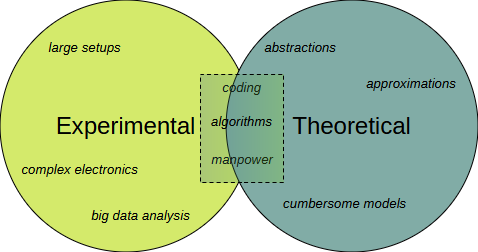
\includegraphics[scale=0.35]{figures/exp_vs_theory.png}
    \end{figure}
\end{frame}


\begin{frame}
	\frametitle{Triaxiality - Nuclear facilities}
	\begin{columns}
		\column{0.4\textwidth}
		\begin{figure}
		\centering
		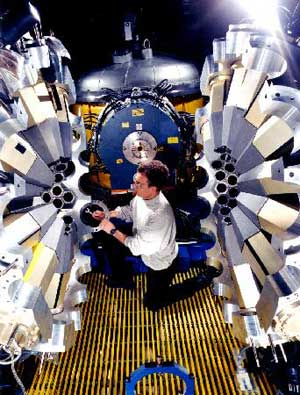
\includegraphics[width=0.86\textwidth]{figures/gsfig.jpg}
		\caption{Gammasphere detector, ANL-ATLAS USA. \textit{Source: aps.org}}
	\end{figure}
	\column{0.6\textwidth}
	\begin{figure}
		\centering
		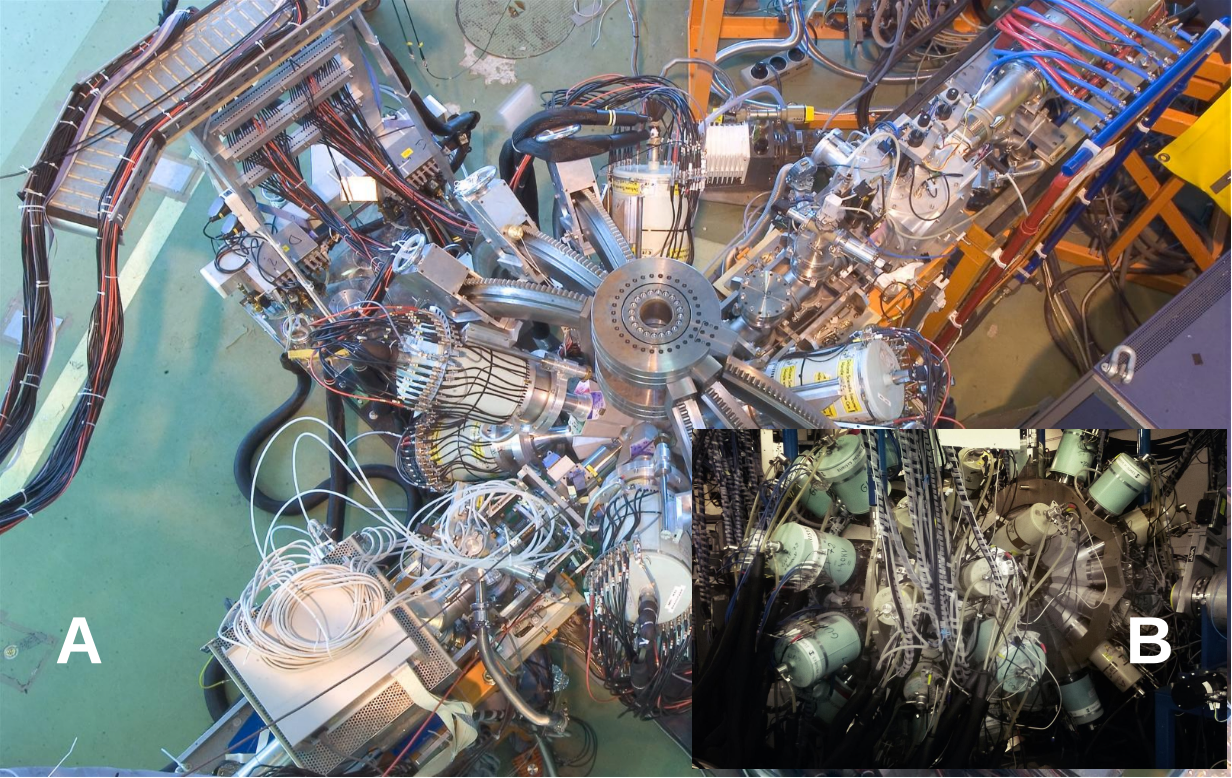
\includegraphics[width=0.98\textwidth]{figures/isolde_cern_2.png}
		\caption{a) IDS detector, CERN. \textit{Source: isolde.web.cern.ch} b) JUROGAM II, Finland. \textit{Source: twitter.com}}
		\end{figure}
	\end{columns}
\end{frame}

\section{Introduction}

\begin{frame}
    \transduration<0-5>{0}
    \multiinclude[<+->][format=png, graphics={width=\textwidth}]{figures/wobbler-gif/wobbler}
    % \animategraphics[loop,controls,width=\linewidth]{10}{figures/wobbler-gif/wobbler-}{0}{5}
\end{frame}

\subsection{Nuclear Shapes}
\begin{frame}
    \frametitle{Text}
    Text
\end{frame}
\subsection{Nuclear Triaxiality}
\begin{frame}
    \frametitle{Text}
    Text
\end{frame}
\subsection{Wobbling Motion}
\begin{frame}
    \frametitle{Text}
    Text
\end{frame}

\begin{frame}[plain] % The optional argument 'plain' hides the headline and footline
	\begin{center}
		\bigskip\bigskip % Vertical whitespace
		{\Huge Thank you for your attention \faHeart}
	\end{center}
\end{frame}

\end{document}
